\documentclass[tikz, convert=pdf2svg]{standalone}
\usetikzlibrary{positioning, backgrounds}
\begin{document}
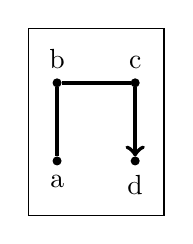
\begin{tikzpicture}[framed]
    \node[draw, inner sep=1pt, circle, fill, label=below:{a}] (a) {};
    \node[draw, inner sep=1pt, circle, fill, label={b}, above=25pt of a] (b) {};
    \node[draw, inner sep=1pt, circle, fill, label={c}, right=25pt of b] (c) {};
    \node[draw, inner sep=1pt, circle, fill, label=below:{d}, below=25pt of c] (d) {};

    \draw[->, line width=1.5pt] (a) -- (b) -- (c) -- (d);


\end{tikzpicture}
\end{document}
